\begin{yl}{4}{Sipelgas}{sipelgas}{1 sekund}{40 punkti}
  \emph{Idee ja teostus: Heno Ivanov, lahenduse selgitus: Ahto Truu}

  \begin{quote}
    Kuubi tipus seisev robotsipelgas liigub käsu \verb|V| peale järgmisse tippu mööda endast vasakul olevat, käsu \verb|P| peale mööda paremal olevat serva. Sipelga täidetud käskude jada põhjal leida lühima võimalik tee tagasi algustippu.
  \end{quote}

Ülesanne leida lühim tee peaks mõtted kohe graafidele viima. Graafiülesandena lahendamiseks peame tähele panema, et sipelga olekus on lisaks tema asukohale oluline ka tema pea suund, milleks kuubi igas tipus on kolm võimalust.

\begin{center}
  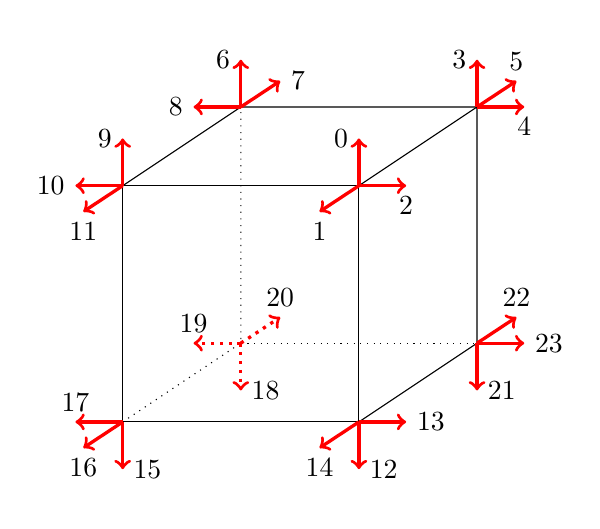
\begin{tikzpicture}
    \draw[white] (-1, -1) -- (5.5, -1) -- (5.5, 5) -- (-1, 5) -- (-1, -1);
    \draw (0, 0) -- (3, 0) -- (3, 3) -- (0, 3) -- (0, 0);
    \draw (3, 0) -- (4.5, 1) -- (4.5, 4) -- (3, 3);
    \draw (4.5, 4) -- (1.5, 4) -- (0, 3);
    \draw[dotted] (0, 0) -- (1.5, 1) -- (1.5, 4);
    \draw[dotted] (1.5, 1) -- (4.5, 1);

    \draw[->, red, very thick] (3, 3) -- (3, 3.6) node[left, black]{0};
    \draw[->, red, very thick] (3, 3) -- (2.5, 2.67) node[below, black]{1};
    \draw[->, red, very thick] (3, 3) -- (3.6, 3) node[below, black]{2};

    \draw[->, red, very thick] (4.5, 4) -- (4.5, 4.6) node[left, black]{3};
    \draw[->, red, very thick] (4.5, 4) -- (5.1, 4) node[below, black]{4};
    \draw[->, red, very thick] (4.5, 4) -- (5, 4.33) node[above, black]{5};

    \draw[->, red, very thick] (1.5, 4) -- (1.5, 4.6) node[left, black]{6};
    \draw[->, red, very thick] (1.5, 4) -- (2, 4.33) node[right, black]{7};
    \draw[->, red, very thick] (1.5, 4) -- (0.9, 4) node[left, black]{8};

    \draw[->, red, very thick] (0, 3) -- (0, 3.6) node[left, black]{9};
    \draw[->, red, very thick] (0, 3) -- (-0.6, 3) node[left, black]{10};
    \draw[->, red, very thick] (0, 3) -- (-0.5, 2.67) node[below, black]{11};

    \draw[->, red, very thick] (3, 0) -- (3, -0.6) node[right, black]{12};
    \draw[->, red, very thick] (3, 0) -- (3.6, 0) node[right, black]{13};
    \draw[->, red, very thick] (3, 0) -- (2.5, -0.33) node[below, black]{14};

    \draw[->, red, very thick] (0, 0) -- (0, -0.6) node[right, black]{15};
    \draw[->, red, very thick] (0, 0) -- (-0.5, -0.33) node[below, black]{16};
    \draw[->, red, very thick] (0, 0) -- (-0.6, 0) node[above, black]{17};

    \draw[->, red, very thick, dotted] (1.5, 1) -- (1.5, 0.4) node[right, black]{18};
    \draw[->, red, very thick, dotted] (1.5, 1) -- (0.9, 1) node[above, black]{19};
    \draw[->, red, very thick, dotted] (1.5, 1) -- (2, 1.33) node[above, black]{20};

    \draw[->, red, very thick] (4.5, 1) -- (4.5, 0.4) node[right, black]{21};
    \draw[->, red, very thick] (4.5, 1) -- (5, 1.33) node[above, black]{22};
    \draw[->, red, very thick] (4.5, 1) -- (5.1, 1) node[right, black]{23};
  \end{tikzpicture}
\end{center}

Kui nummerdame olekud nii, nagu näidatud ülaloleval joonisel, ja kirjutame iga oleku jaoks välja, millisesse olekusse sipelgas sealt kummagi käsuga edasi liigub, on juba lihtne koostada ka funktsioon, mis leiab algolekust mingite käskude täitmise järel saadud lõppoleku:

\begin{tabular}{p{\colwidth} p{\colwidth}}
Python:
\begin{lstlisting}[language=Python]
vasakule = [
  10, 12,  5,  1, 21,  8,
   4, 18, 11,  7, 15,  2,
  22,  0, 17, 13,  9, 20,
  16,  6, 23, 19,  3, 14]
paremale = [
   5, 10, 12,  8,  1, 21,
  11,  4, 18,  2,  7, 15,
  17, 22,  0, 20, 13,  9,
  23, 16,  6, 14, 19,  3]

def liigu(olek, sammud):
  for samm in sammud:
    if samm == 'V':
      olek = vasakule[olek]
    if samm == 'P':
      olek = paremale[olek]
  return olek
\end{lstlisting}
&
C++:
\begin{lstlisting}[language=C++]
vector<int> vasakule = {
  10, 12,  5,  1, 21,  8,
   4, 18, 11,  7, 15,  2,
  22,  0, 17, 13,  9, 20,
  16,  6, 23, 19,  3, 14};
vector<int> paremale = {
   5, 10, 12,  8,  1, 21,
  11,  4, 18,  2,  7, 15,
  17, 22,  0, 20, 13,  9,
  23, 16,  6, 14, 19,  3};

int liigu(int olek, string sammud) {
  for (auto samm : sammud) {
    if (samm == 'V') {
      olek = vasakule[olek];
    }
    if (samm == 'P') {
      olek = paremale[olek];
    }
  }
  return olek;
}
\end{lstlisting}
\end{tabular}

Tagasitee võiksime muidugi leida mõne standardse lühima tee leidmise algoritmiga. Aga saab ka lihtsamalt, kui paneme tähele, et mistahes tipust mistahes teise tippu saab alati ülimalt kolme sammuga. See tähendab, et võimalikke tagasiteid pole kuigi palju ja võime kõik variandid lihtsalt programmi sisse kirjutada:

\begin{tabular}{p{\colwidth} p{\colwidth}}
Python:
\begin{lstlisting}[language=Python]
teed = [
  "",
  "V", "P",
  "VV", "VP", "PV", "PP",
  "VVV", "VVP", "VPV", "VPP",
  "PVV", "PVP", "PPV", "PPP"]
\end{lstlisting}
&
C++:
\begin{lstlisting}[language=C++]
vector<string> teed = {
  "",
  "V", "P",
  "VV", "VP", "PV", "PP",
  "VVV", "VVP", "VPV", "VPP",
  "PVV", "PVP", "PPV", "PPP"};
\end{lstlisting}
\end{tabular}

Õigupoolest saaks ka nendest nimekirjadest veel mitmeid variante välja jätta. Näiteks peaks olema lihtne näha, et mistahes olekust alustades jõuame käsujadade \lstinline[language=Python]|"VP"| ja \lstinline[language=Python]|"PV"| järel alati samasse tippu (kuigi mitte samasse olekusse). Aga siiski on need nimekirjad juba praegu piisavalt lühikesed, et on triviaalne kõik variandid läbi proovida ja esimene lähtetippu tagasi viiv variant vastusena välja trükkida:

\begin{tabular}{p{\colwidth} p{\colwidth}}
Python:
\begin{lstlisting}[language=Python]
_ = int(input())
tee = input().strip()
olek = liigu(0, tee)

for tee in teed:
  if liigu(olek, tee) in [0, 1, 2]:
    print(len(tee))
    print(tee)
    break
\end{lstlisting}
&
C++:
\begin{lstlisting}[language=C++]
int main() {
  int n;
  cin >> n;
  string tee;
  cin >> tee;

  int olek = liigu(0, tee);
  for (auto tee : teed) {
    int lopp = liigu(olek, tee);
    if (lopp == 0 or lopp == 1 or lopp == 2) {
      cout << tee.length() << '\n';
      cout << tee << '\n';
      break;
    }
  }
}
\end{lstlisting}
\end{tabular}


\end{yl}
